\documentclass[a4paper, 10pt]{article}
\usepackage[utf8]{inputenc}
\usepackage[spanish] {babel}
\usepackage{amsfonts}
\usepackage{amssymb}
\title{Trabajo Practico 1}
\usepackage{tpalgo3}
\usepackage{caratula}
\usepackage{amssymb}
\usepackage[pdftex]{graphicx}
\usepackage{hyperref}

\setlength{\leftmargin}{10cm}
\setlength{\rightmargin}{10cm}
\setlength{\oddsidemargin}{-1cm}
\setlength{\evensidemargin}{-1cm}
\setlength{\topmargin}{-1cm}
\setlength{\textwidth}{18cm}
\setlength{\textheight}{25cm}

\usepackage{fancyhdr}
\pagestyle{fancy}
\fancyhf{}
\fancyhead [L]{\scriptsize Trabajo Práctico N$^{\circ}$1}
\fancyhead [R]{\scriptsize Aronson, Garbi, Nahabedian, Ravesi}%1{20pt}
\fancyfoot[C]{\thepage}
\renewcommand{\footrulewidth}{0.4pt}

\begin{document}
\materia{Algoritmos y Estructuras de Datos III}
\submateria{Primer Cuatrimestre de 2010}
\titulo{Trabajo Practico N$^{\circ}$1}
\grupo{Grupo 14}
\integrante{Aronson Alex}{443/08}{aronsonalex@hotmail.com}
\integrante{Garbi Sebastián Lionel}{179/05}{garbyseba@hotmail.com}
\integrante{Nahabedian Leandro Ezequiel}{250/08}{leanahabedian@hotmail.com}
\integrante{Ravasi Nicolás Martín}{53/08}{nravasi@gmail.com}
\maketitle
\newpage

\tableofcontents
\newpage

\section{Archivos entregados en este TP}

En la entrega de este TP, los archivos están separados en carpetas según el ejercicio. Los archivos fuente principales, los cuales generan el binario que resuelve correctamente cada ejercicio, son $ej1.cpp$, $ej2.cpp$ y $ej3.cpp$, localizados en su respectiva carpeta. Además, cada una cuenta con un $timer.cpp$ que muestra la cantidad de operaciones efectuadas por cada ejercicio. En el caso de los dos primeros, se cuenta con un $rangen.cpp$, que genera un input al azar, y en el 1 con un $peorcaso.cpp$ que genera el peor caso. Todos los cpp se compilan y generan un ejecutable simplemente con el Makefile que se encuentra en dicha carpeta.

Además, se incluyen archivos de input llamados $input.txt$, y en el caso del ejercicio 3, un $peorcaso.txt$ adicional.

\section{Ejercicio 1}

\subsection{Enunciado}

Un conjunto de intervalos $\{[x_1 , y_1 ], ..., [x_n , y_n ]\}$ cubre al intervalo $[0, M ]$ si y solo si para cada entero
$0 \le a \le M$ , hay un $i$ tal que $a \in [x_i , y_i ]$. En este problema, dado $M$ y un conjunto de intervalos, se debe
seleccionar un subconjunto de cardinal mínimo de esos intervalos que cubran el intervalo $[0, M ]$.

\subsection{Breve descripción del algoritmo}

Para este problema encaramos la solución construyendo con los datos de entrada una lista, la cual pasamos como parámetro a la función que resuelve el problema. En ésta, primero hacemos un sort que ordena en primer lugar por la primera coordenada del par (o sea, el límite por debajo del intervalo) y en caso de igualdad por la segunda. Una vez hecho esto, procedemos a eliminar los pares cuya primera coordenada sea igual, dejando sólo el mismo de mayor segunda coordenada, pasando estos elementos a un nuevo vector.

Luego, recorremos este vector secuencialmente buscando primero hasta una coordenada que sea mayor que 0, guardando siempre el valor máximo encontrado en la segunda coordenada de los pares recorridos. Una vez encontrado (en caso negativo, salimos del algoritmo), pusheamos este intervalo en la salida y procedemos a la parte principal del algoritmo, donde recorremos los elementos hasta encontrar uno cuya primera coordenada sea mayor a la segunda del último intervalo pusheado, siempre guardando la segunda coordenada máxima y su posición, una vez alcanzado, se pushea dicha posición y se continúa de la misma manera.

Esto lo hacemos o bien hasta que no podamos seguir, en cuyo caso devuelve negativo, o bien hasta llegar al objetivo pedido, en cuyo caso devolvemos la lista construida.\\


\nuevoAlgo{Algoritmo 1}{minCantDeIntervalos($intervalos$ : $vector<tupla<Nat,Nat>>$, $M$ : $Nat$)} $\rightarrow$ $res$ :
$vector<tupla>$ .
Dado un conjunto de intervalos y un natural $M$, devuelve la cantidad mínima de intervalos tal que el intervalo $[0..M]$ queda completamente cubierto.\} \\

\begin{tabular}{rp{17cm}}
1: & minCantDeIntervalos ($intervalos$ : $vector<tupla<Nat,Nat>>$, $M$ : $Nat$)\ \{\\
2: & \hspace{0,5cm}   \asignar{res : vector<tupla<Nat,Nat>>}{Vacio} \\
3: & \hspace{0,5cm}   \asignar{intervalos}{ordenar(intervalos)}\\
4: & \hspace{0,5cm}   \asignar{filtrados : vector<tupla<Nat,Nat>>}{filtrarDejandoIntervalosMasGrandes(intervalos)}\\
5: & \hspace{0,5cm}   \asignar{objetivo : Nat}{0} \\
6: & \hspace{0,5cm}   \asignar{maximo : tupla<Nat,Nat>}{Vacia} \\
7: & \hspace{0,5cm}   $\forall$ par\ $\in\ $ filtrados\ \{\\
8: & \hspace{1cm}         $\mientras$ ($\pi_1$(par) $<$ objetivo ) \{ \\
9: & \hspace{1,5cm}           \iif $(\pi_2(par) < \pi_2(maximo))$ $=>$ (\asignar{maximo}{par})\\
10: & \hspace{1cm}        \} \\
11: & \hspace{1cm}        \iif noHayIntervalo(objetivo)\}\\
12: & \hspace{1,5cm}      	  \devolver 0\\
13: & \hspace{1cm}        objetivo $\gets$ $\pi_2$(maximo)\\
14: & \hspace{1cm}		  res.insertar(maximo) \\
15: & \hspace{1cm}        \iif llegueA?(M, objetivo) \\
16: & \hspace{1,5cm}         \devolver res\\
17: & \hspace{1cm}        \finif \\
18: & \hspace{0,5cm}  \} \\
19: & \hspace{0,5cm}  \devolver  0\\
20: & \}\\ \\
\end{tabular}
\\
La operación ordenar es la llamada a $sort()$ del contenedor $list$ de la librería de $C++$.\\
La función $filtrarDejandoIntervalosMasGrandes()$ recibe un conjunto de intervalos y se encarga de sacar aquellos
$[x,y]$ donde $x = y$ o aquellos tal que existe otro intervalo $[p,q]$ donde $p = x$ y $q \geq y$.\\
$noHayIntervalo()$ recibe como parámetro el valor que se quiere cubrir mediante un próximo intervalo. Si no se encontró
alguno que cubra dicho número, devuelve false.\\
Por ultimo la llamada a la función $llegueA?()$ recibe el $M$ y el próximo valor el cual quiero cubrir. Si este ultimo es
mayor entonces $M$ ya fue cubierto y obtendremos un true como resultado de esta operación.



\subsection{Correctitud}

Para demostrar que la solución obtenida es realmente la solución del problema, se puede decir que primero, luego de hacer $sort()$ por primera coordenada, se filtran todos aquellos intervalos que de ninguna manera podrían ser parte de la solución, ya que existe al menos un intervalo cuya primera coordenada es la misma y con una mayor segunda coordenada. Una vez hecho esto, sabiendo que está ordenado, recorremos desde el principio hasta llegar a un intervalo cuyo inicio sea mayor que 0, y nos quedamos con el intervalo de mayor segunda coordenada de los recorridos hasta entonces si los hubiere; esto se hace porque es necesario encontrar un intervalo que empiece con 0 o un número negativo, y de esos elegimos el de mayor alcance, que es el mejor candidato (si no hay candidato, entonces no hay solución y por eso salimos del algoritmo)

Luego, procedemos a recorrer los intervalos hasta llegar a la segunda coordenada guardada, o sea, hasta cubrir el máximo espectro posible con los intervalos ya seleccionados. Una vez recorridos, seleccionamos el de mayor segunda coordenada nuevamente, o sea, siempre elegimos aquel que llega más lejos de manera de minimizar la cantidad de intervalos usados; como siempre elegimos aquel que cubra más territorio, y siempre cubrimos todo el espectro posible, se desprende que no puede haber un intervalo no elegido que cubra más números o que cause que se reduzca la cantidad de intervalos de salida, porque si así fuera, la naturaleza misma de nuestro algoritmo goloso hubiera causado que fuera elegido en esa instancia.

\subsection{Complejidad}

La restricción de eficiencia que debíamos cumplir para este ejercicio era que la complejidad algorítmica sea estrictamente menor que $n^2$. Para probar que realmente cumplimos con esa cota analicemos el pseudocódigo:

\begin{tabular}{rp{15.8cm}}
2:& Creo un vector con ningún elemento dentro, esta operación es constante.\\
3:& El vector recibido como parámetro lo ordenamos usando la función $sort()$\footnotemark de la librería de $C++$. Ordena de acuerdo a la primera coordenada y luego en base a la segunda. El costo de esta instrucción es $n log(n)$. Debemos tener cuidado porque en este caso ordenamos pares y no números. De todos modos la complejidad no se altera ya que son siempre tuplas de 2 elementos. Luego este paso tiene un costo de $O(n * log(n))$.\\
4:& Ejecutamos la función $filtrarDejandoIntervalosMasGrandes(intervalos)$, que se encarga de sacar aquellos intervalos
$[x,y]$ donde $x = y$ o aquellos tal que existe otro intervalo $[p,q]$ donde $p = x$ y $q \geq y$. Realizar este filtro tiene
costo lineal porque hay que recorrer todo el vector chequeando estas condiciones. Por lo tanto esta instrucción es del orden de $O(n)$.\\
5 y 6:& Son operaciones básicas de costo constante.\\
7:& Iniciamos un ciclo. Este va a recorrer los intervalos ya filtrados. En el peor caso, nuestro filtro no hizo nada, y por lo tanto ejecutaríamos las próximas instrucciones $n$ veces.\\
8-10:& Lo que pedimos en estos pasos es que de todos aquellos intervalos que cumple la propiedad de que el numero objetivo esta en el intervalo, danos el que más lejos llega. Este conjunto de instrucciones no es mas que seguir hacia adelante en el loop descripto en el paso 7 porque como el vector de intervalos esta ordenado, el máximo de todos los intervalos que contienen el objetivo esta mas adelante que el actual. El costo de esto, es hacer las asignaciones y comparaciones descriptas en el pseudocódigo. Por lo tanto son constantes.\\
11 y 12:& En este paso trato de verificar si caímos en un caso donde no hay solución. Para esto tengo que chequera si el objetivo sigue siendo el mismo y luego devuelvo $0$. Esto tiene una complejidad constante.\\
13:& Cambio de valor de objetivo por el nuevo objetivo, que es la segunda coordenada de $maximo$. Es una asignación por lo tanto constante.\\
14:& Insertamos un elemento utilizando la instrucción $push\_back()$\footnotemark de la librería $C++$. Pushear una tupla es constante.\\
15-20:& Son todas operaciones constantes, chequear si alcanzamos el $M$ devolver el vector con los intervalos resultados o devolver $0$ en caso de no llegar a $M$ por ningún camino.\\
\end{tabular}

\footnotetext[1]{http://www.cplusplus.com/reference/stl/list/sort/}
\footnotetext[2]{http://www.cplusplus.com/reference/stl/list/push\_back/}

Luego podemos observar que la complejidad de este algoritmo, en base a $n$ intervalos recibidos como parámetro, esta compuesta por: $O(n * log(n))$ del $sort()$, $O(n)$ para filtrar los intervalos y la ejecución de un ciclo que itera $n$ veces sobre operaciones constantes, formando un costo $O(n)$

Finalmente podemos afirmar que nuestro algoritmo es del orden de:
\begin{center}
$O(n * log(n)) + O(n) + O(n) = O(max\{n * log(n), 2n\}) \in O(n * log(n))$
\end{center}



\subsection{Casos de Pruebas y Gráficos}

Para los casos de prueba, creamos dos generadores de caso, uno, $rangen.cpp$ que generara inputs al azar de tamaño especificado por nosotros (el cual fuimos variando al hacer el testeo); el otro, $peorcaso.cpp$, crea un input en el que se cubre el intervalo pedido con intervalos de tamaño 1, de manera que el algoritmo tenga que recorrer toda la entrada y no se puedan descartar repetidos. Para hacer las mediciones, decidimos contar la cantidad de operaciones llevadas a cabo, usando $n* log (n)$ en el caso de la función sort (con $n$ la cantidad de intervalos). Esto se calcula con $timer.cpp$, el cual devuelve por salida estándar la cantidad de operaciones llevadas a cabo, estos datos los volcamos en la tabla y gráfico siguientes.


\begin{center}
\begin{tabular}{|c|c|c|c|}
\hline
\# Tamaño de la entrada & Cantidad experimental de operaciones & Caso Teórico: 10.2$*$n log n & Peor caso\\
\hline
30 & 352 & 452 & 344\\
\hline
72 & 1,341 & 1,364 & 885\\
\hline
100 & 1,868 & 2,040 & 1,262\\
\hline
541 & 7,692 & 15,082 & 7,734\\
\hline
1,000 & 14,727 & 30,600 & 14,909\\
\hline
4,703 & 73,306 & 176,166 & 77,394\\
\hline
10,000 & 169,698 & 408,000 & 172,105\\
\hline
57,033 & 1,045,805 & 2,766,813 & 1,080,856\\
\hline
100,000 & 1,860,623 & 5,100,000 & 1,951,294\\
\hline
423,354 & 9,625,965 & 24,297,293 & 8,871,793\\
\hline
1,000,000 & 21,077,828 & 61,200,000 & 21,815,512\\
\hline
4,711,243 & 112,574,288 & 320,675,382 & 110,080,372\\
\hline
10,000,000 & 231,531,187 & 714,000,000 & 241,180,958\\
\hline
\end{tabular}
\end{center} \vspace{0,15cm}


\begin{center}
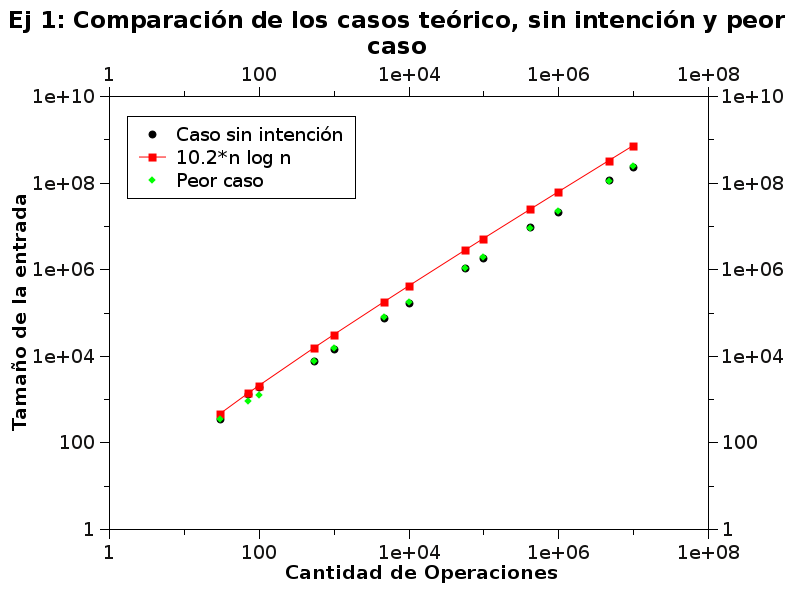
\includegraphics[scale=0.60]{graficos/1-ej.png} \\
\scriptsize{\textsf{\textbf{Gr\'afico 1.1}}}  \\
\end{center}

\newpage
\section{Ejercicio 2}

\subsection{Enunciado}

La mediana de un conjunto de un conjunto de $n$ números $x_1 < x_2 < ... < x_n$ se define como $x_{(n+1)/2}$ si $n$ es impar,
o como $(x_{n/2} + x_{n/2+1} )/2$ si $n$ es par. Dados $n$ números enteros en cualquier orden $y_1 , ..., y_n$ se deben
devolver otros $n$ números, donde el i-ésimo de ellos represente la parte entera de la mediana de los primeros $i$ números de
la entrada $y1, ..., yi$.

\subsection{Breve descripción del algoritmo}

\nuevoAlgo{Algoritmo 2}{hallarMedianas ($numeros$ : $vector<Nat>$)} $\rightarrow$ $res$ : $vector<Nat>$.
Devuelve tantos números como la entrada posee, que representa, para cada $i$ entre 0 y $n$, la parte entera de la mediana
desde $numeros_0$ hasta $numeros_i$.\} \\

\begin{tabular}{rp{17cm}}
1: & hallarMedianas ($numeros$ : $vector<Nat>$)\ \{\\
2: & \hspace{0,5cm}   \asignar{res : vector<Nat>}{Vacio} \\
3: & \hspace{0,5cm}   \asignar{menores : ColaPrioridad<Nat>}{Vacio}\\
4: & \hspace{0,5cm}   \asignar{mayores : ColaPrioridad<Nat>}{Vacio} \\
5: & \hspace{0,5cm}   $\forall\ entero\ \in\ numeros$\ \{\\
6: & \hspace{1cm}         medio : Nat $\gets$ OrdenarColas(entero, menores, mayores) \\
7: & \hspace{1cm}         \iif $(esPar(\#(numeros)))$\\
8: & \hspace{1,5cm}           $res.insertar((max(menores) + min(mayores)) /2)$\\
9: & \hspace{1cm}         \sino \\
10: & \hspace{1,5cm}          $res.insertar(medio)$ \\
11: & \hspace{1cm}        \finif\\
12: & \hspace{1cm}        \} \\
13: & \hspace{1cm}        \devolver res \\
14: & \}\\ \\
\end{tabular}
\\

La función ordenarColas($entero$, $menores$, $mayores$) devuelve, en caso de que $i$ es impar, el
elemento tal que existen $h$ números por debajo de él y otros $h$ por encima, a su vez ordena las colas para lograr las complejidades. Siendo $h$ $\in$ $[0 \lfloor n/2\rfloor]$.
Si estoy en una iteración donde $i$ es par entonces a medio se le asigna un 0.
Para implementar las colas  usamos priority\_queues de la libreria de C$++$, usando un max-heap (o sea, una cola donde el tope es el máximo de la misma) para los valores menores que la mediana y un min-heap para los mayores.
Además vale que la \#($menores$) == \#($mayores$) al terminar cada iteración.


\subsection{Correctitud}

Para realizar el análisis de porque nuestro algoritmo es correcto, es necesario ver que devolvemos la respuesta correcta en
el primer paso del ciclo y sigue siendo correcto a traves de las iteraciones.\\

\hspace{-0,5cm} \underline{Primera iteración:}\\

Veamos que la función ordenarColas() me devuelve el numero que tiene igual cantidad de números por debajo y por encima de él. Al principio tengo un único numero, por lo tanto hay 0 elementos menores y 0 mayores. Por lo tanto, el valor de la variable $medio$ es igual al primer elemento del vector $numeros$. Luego, nuestro algoritmo, como hay impar elementos coloca en el vector $res$ la variable $medio$. La mediana de un solo elemento, es el elemento propiamente dicho, por lo tanto el vector res tiene la respuesta correcta en su primera posición para el primer elemento.\\


\hspace{-0,5cm} \underline{Iteración $i$:}\\

Para esta etapa sé que nuestro algoritmo es correcto hasta $i-1$ elementos previos.
Además en este paso vale que los elementos de $mayores$ $\cup$ $menores$ $\cup$ $\{medio\}$ son los mismos que los primeros $i-1$ elementos del vector pasado como parámetro.

Lo separaremos en 2 casos: si hay cantidad par de elementos o hay cantidad impar, al agregar el i-ésimo.\\\\
Si $i$ es impar: \\

Cuando agregamos un elemento ajustamos los valores de $medio$, $mayores$ y $menores$ con la función ordenarCola() procurando que en $medio$ haya un valor mayor o igual a todos los que viven en $menores$ y menor o igual a todos los que viven en $mayores$.
Luego, hay $\lfloor i/2\rfloor$ elementos menores que la variable $medio$ e $\lfloor i/2\rfloor$ elementos mayores.
Además, se ejecuta la instrucción $res.insertar(medio)$ que deja en la posición i-esima del vector $res$ el valor de la variable $medio$, que es exactamente la mediana hasta el i-ésimo elemento, ya que $medio$ tiene tantos números por debajo como números por encima para este caso donde la cantidad total de elementos es impar.\\\\

\noindent Si $i$ es par:\\

Sea $V$ el arreglo dado por los primeros $i$ elementos del vector pasado como parámetro, y esta ordenado\\
Como hay cantidad par, la mediana del vector $V$ es igual a $(V_{i/2 -1} + V_{i/2}) /2$.
Efectivamente es lo que nuestro algoritmo almacena en la posición $i$ del vector $res$, ya que nosotros colocamos en esa posición el valor de $(max(menores) + min(mayores)) /2$.
Probemos que $max(menores)$ contiene el mismo valor que $V_{i/2 -1}$\\
y que $min(mayores)$ contiene el mismo valor que $V_{i/2}$.\\
Como $V$ esta ordenado los anteriores a $V_{i/2 -1}$ son los números mas chicos de $V$ y menores o iguales que $V_{i/2 -1}$.
Esta propiedad vale también para $max(menores)$ porque en $menores$ tengo los $i/2$ números mas chicos y tomo el mas grande
de ellos.\\
Lo mismo pero al revés pasa con $V_{i/2}$. Los siguientes a este son los números mas grandes de $V$ y mayores o iguales que $V_{i/2}$ que es equivalente a obtener el min() de $mayores$ que posee siempre los $i/2$ elementos mas grandes.\\

\noindent Finalmente como los $n$ resultados los fuimos almacenando en el vector $res$, entonces $res$ es la solución del problema y nuestro algoritmo es correcto.

\subsection{Complejidad}

El enunciado del problema pedía que la complejidad algorítmica sea estrictamente mejor que $n^2$
para cumplir con esto analicemos el pseudocódigo:\\

\begin{tabular}{rp{15.8cm}}
2-4: & Se inicializan vectores y heaps, el costo es constante\\
5-12:& Realizamos un ciclo que recorre el vector pasado como parámetro, el código de las lineas
entre 5 y 12 se ejecutan $n$ veces, con $n$ igual a la cantidad de elementos del arreglo pasado como
parámetro\\
6: & Se ejecuta la función $ordenarColas()$. Dependiendo de como se ordenan los heaps, se realizaran diferentes operaciones, pero podemos afirmar que los peores casos son cuando agrego un elemento en cada heap, o cuando tengo que sacar el tope de un heap y agregarle otro valor. Las operaciones usadas son dos llamados a $push()$\footnotemark en el primer caso, o una llamada a $pop()$\footnotemark y luego a $push()$. Estas operaciones son operaciones incluidas en la librería estándar de $C++$ y el costo de cada una es del orden logaritmico. Como los heaps en cada iteración tienen $\lfloor i/2\rfloor$ cantidad de elementos. El costo de esta instrucción, en el peor caso es de es $O(log \lfloor n/2\rfloor + log \lfloor n/2\rfloor) = O(2* log \lfloor n/2\rfloor) =
O(log \lfloor n/2\rfloor)$ \\
7: & La cantidad de elementos la tenemos guardada en una variable, por lo tanto hallar la paridad de la cantidad de números es constante.\\
8-12: & Para agregar al final del vector $res$ un valor usamos la operación push\_back() de listas implementado en la librería de $C++$ que es constante.\\
13: & Devolvemos el vector $res$ como solución a nuestro problema, se realiza en tiempo constante.\\
\end{tabular}
\\\\

\footnotetext[3]{http://www.cplusplus.com/reference/stl/priority\_queue/push/}
\footnotetext[4]{http://www.cplusplus.com/reference/stl/priority\_queue/pop/}

Finalmente la complejidad de nuestro algoritmo ejecuta $n$ veces la operación ordenarColas() que según lo
explicado anteriormente tiene complejidad $O(log \lfloor n/2\rfloor)$

Luego, la complejidad es de:
\begin{center}
$O(n) * O(log \lfloor n/2\rfloor) \in O(n * log(n))$
\end{center}


\subsection{Casos de prueba y Gráficos}

Teniendo en cuenta que no encontramos un peor caso para este ejercicio (ver más abajo), creamos un programa $rangen.cpp$ que generara inputs al azar de tamaño especificado por nosotros (el cual fuimos variando al hacer el testeo). Para hacer las mediciones, decidimos contar la cantidad de operaciones llevadas a cabo, usando log (cantidad de elementos en el heap) en el caso de los push y pop. Esto se calcula con $timer.cpp$, el cual devuelve por salida estándar la cantidad de operaciones llevadas a cabo, estos datos los volcamos en la tabla y gráfico siguientes.

\begin{center}
\begin{tabular}{|c|c|c|}
\hline
\# Tamaño de la entrada & Cantidad experimental de operaciones & Caso Teórico: 7*n log n\\
\hline
10 & 67	& 70\\
\hline
58 & 521 & 716\\
\hline
100 & 986 & 1,400\\
\hline
574 & 7,154 & 11,085\\
\hline
1,000 & 13,304 & 21,000\\
\hline
4,988 & 78,440 & 129,117\\
\hline
10,000 & 167,689 & 280,000\\
\hline
37,888 & 711,117 & 1,214,291\\
\hline
100,000 & 2,022,394 & 3,500,000\\
\hline
664,789 & 15,332,746 & 27,095,993\\
\hline
1,000,000 & 23,676,892 & 42,000,000\\
\hline
3,545,210 & 90,667,215 & 162,538,993\\
\hline
10,000,000 & 271,296,349 & 490,000,000\\
\hline
\end{tabular}
\end{center} \vspace{0,15cm}

Como se puede observar a medida que aumentamos el tamaño de la entrada, la cantidad de comparaciones que realiza nuestro algoritmo nunca supera la complejidad teórica y la distribución de puntos sigue la función $c*n * log(n)$ donde $c$ resulto ser 7 en la práctica.


\begin{center}
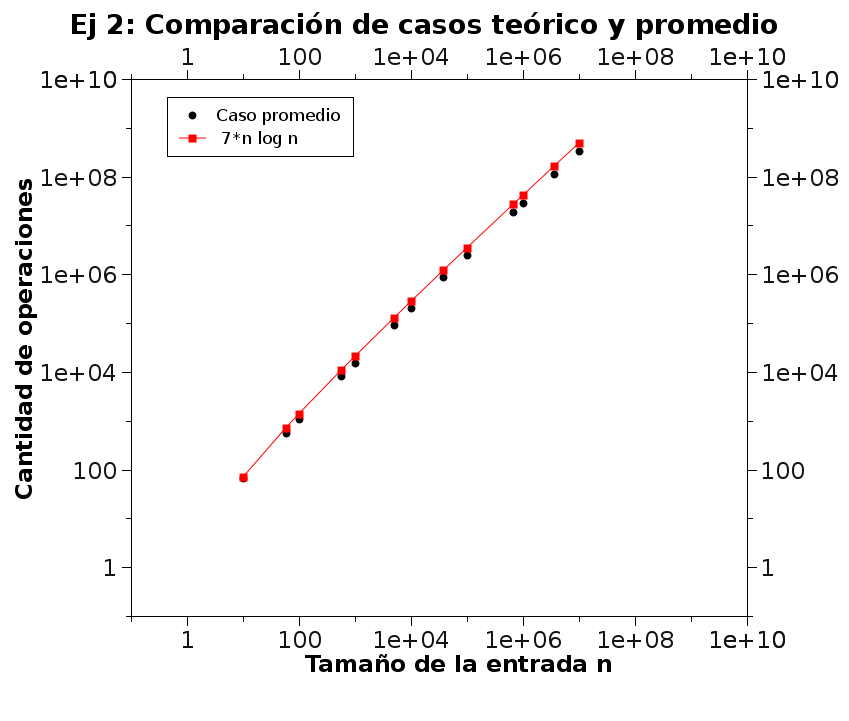
\includegraphics[scale=0.50]{graficos/2-ej.png} \\
\scriptsize{\textsf{\textbf{Gr\'afico 2.1}}}  \\
\end{center}

Para este ejercicio tratamos de encontrar un peor caso el cual generara una mayor cantidad de operaciones, pero dada la naturaleza del algoritmo, siempre se hacen las mismas operaciones para los casos pares e impares, sin importar demasiado los valores de la entrada. Si bien es lógico suponer que el push a los heaps tardaría más en los casos en que tiene que bajar mucho (o sea, si se insertara un elemento muy chico en el maxheap $menores$ o inversamente un elemento muy grande en el minheap $mayores$), esta función no fue codeada por nosotros y por lo tanto no podemos especular sobre cómo actúa la misma.

Por lo tanto, consideramos que en esencia la cantidad de operaciones llevadas a cabo por el algoritmo depende muy poco de los valores de entrada, y por ende descartamos la existencia de un peor caso.

\newpage
\section{Ejercicio 3}

\subsection{Enunciado}

Se tiene un alfabeto (conjunto de caracteres) y un conjunto de parejas entre ellos. La relación de pareja es simétrica.
Se busca escribir dichos caracteres en cierto orden de manera de minimizar la distancia entre la pareja que quedó más
alejada en dicho orden.

\subsection{Breve descripción del algoritmo}

En este algoritmo, primero lo que hacemos es generar las estructuras de soporte que vamos a usar luego para hacer el backtracking. Estas son dos, un diccionario que guarda todas las relaciones entre los caracteres, cuyas claves son caracteres y sus definiciones son conjuntos que contienen todos los caracteres con los que dicha clave tiene relación, y una lista que marca el alfabeto que falta iterar, en principio es todo el alfabeto.

Con esto, llamamos a la función de backtracking, esta función es recursiva y se divide en dos casos, el caso base se da cuando no queda más alfabeto por considerar, en este caso simplemente llama a una función podar que va a elegir el mejor caso, en caso contrario se generan los nuevos candidatos con la función generar, se hace una poda con la función podar y se vuelve a llamar a backtracking, popeando el primer elemento del alfabeto restante.

La función generar simplemente toma todos los candidatos y el próximo caracter a añadir, y genera todas las posibles combinaciones nuevas, insertando primero atrás de la lista y luego moviéndose hacia adelante, para cada elemento candidato. Es importante remarcar que para garantizar el orden alfabético de los candidatos, si el nuevo caracter a agregar (que dada la forma de construir el alfabeto, es siempre posterior lexicográficamente a los ya añadidos) fuera a quedar como el primer elemento en un candidato, lo agregamos a otra lista, que luego concatenaremos a candidatos.

En podar, descartamos los candidatos que son inviables, estos son, los que tienen una relación con una distancia máxima comparada con el mejor candidato (o sea, el que sería la solución si el alfabeto terminara ahí) superior a la cantidad de caracteres que quedan por iterar, ya que no hay forma de que estos se conviertan en los mejores candidatos. Si es la última iteración, no queda alfabeto entonces simplemente se podan todos los que tienen una distancia máxima mayor.

Finalizado todo esto, se devuelve el primer elemento de los candidatos como resultado.\\
\\
\nuevoAlgo{Algoritmo 3}{minimaDistancia ($letras$ : $vector<Char>$)} $\rightarrow$ $res$ : $vector<Nat>$.
Devuelve la lista con las letras ordenadas de forma que la distancia entre las parejas sea mínima y de la solución encontrada, la distancia máxima entre las parejas.\} \\

\begin{tabular}{rp{17cm}}
1: & minimaDistancia ($letras$ : $vector<Char>$)\ \{\\
2: & \hspace{0,5cm}   candidatos : $lista<Char>$ $\gets$ Vacia\\
3: & \hspace{0,5cm}   \iif letras.esVacio?()\\
4: & \hspace{1cm}   	  podar(0)\\
5: & \hspace{0,5cm}   \sino \\
6: & \hspace{1cm}   	  candidatos : $vector<Char>$ $\gets$ generar(prim(letra), candidatos)\\
7: & \hspace{1cm}         letras.sacarPrimero() \\
8: & \hspace{1cm}         podar(longitud(letras))\\
9: & \hspace{1cm}         minimaDistancia(letras)\\
10: & \hspace{0,5cm}   \finif \\
11: & \}\\ \\
\end{tabular}
\\

\nuevoAlgo{Algoritmo 4}{generar ($letra$ : $char$)} $\rightarrow$ $res$ : $lista <lista<char> >$.
se encarga de formar, de acuerdo a las letras que tiene, todas las permutaciones.\} \\

\begin{tabular}{rp{17cm}}
1: & generar ($letra$ : $char$, viejosCandidatos)\ \{\\
2: & \hspace{0,5cm}   \iif NoHabiaCandidatos?(viejosCandidatos)\\
3: & \hspace{1cm} 		  candidatos $\gets$ letra \\
4: & \hspace{0,5cm}   \sino \\
5: & \hspace{1cm}   	  for each list  $\in$ viejosCandidatos()\\
6: & \hspace{1.5cm}   	  candidatos $\gets$ insertarEnTodasPosicionesPosibles(list, letra)\\ 
7: & \hspace{0,5cm}   \finif \\
8: & \}\\ \\
\end{tabular}
\\

\nuevoAlgo{Algoritmo 5}{podar ($restante$ : $nat$)} $\rightarrow$ $res$ : $lista <lista<char> >$.
Saca todos los candidatos inviables de acuerdo con la cantidad de alfabeto restante.\} \\

\begin{tabular}{rp{17cm}}
1: & podar ($restante$ : $nat$)\ \{\\
2: & \hspace{0,5cm}   lista $<nat>$ distancias\\
3: & \hspace{0,5cm}   for each list $\in$ candidatos\\
4: & \hspace{1cm} 		 distancias $\gets$ (calcularDistancia (list)) \\
5: & \hspace{0,5cm}   $nat$ mindist $\gets$ encontrarMinimo (distancias)\\
6: & \hspace{0.5cm}   	  for each list  $\in$ distancias()\\
7: & \hspace{1cm} 		 \iif actual $>$ mindist + restante \{\\
8: & \hspace{1.5cm}   	  sacarActual(candidatos)\\ 
9: & \hspace{1cm}   \finif \\
10: & \}\\ \\
\end{tabular}
\\


\subsection{Correctitud}

Nuestro algoritmo devuelve la solución correcta puesto que el generar crea todas las combinaciones posibles que se pueden dar agregando una letra más a las ya existentes, ya que toma todos los candidatos y con cada uno genera n+1 candidatos, siendo $n$ la longitud de ese candidato. Estos nuevos candidatos se generan a partir de insertar la nueva letra en cada posición posible sobre la lista vieja. Es por esto que luego de generar se tienen $(n+1)*\#(candidatosAnterior)$, se puede ver que, si no hubiera poda, hacia el final de la recursión tendríamos $n!$ candidatos, con n la longitud del alfabeto, o sea, todos los candidatos posibles.

También vale la pena recalcar que la forma de generar los candidatos hace que estos queden en orden alfabético, puesto que el alfabeto se toma ordenado y los nuevos caracteres se insertan de atrás hacia adelante, más aún, cuando se debería insertar la nueva letra al principio de la lista, como esto causaría que se alterara el orden alfabético si no tuviéramos en cuenta este caso como un caso especial, estos candidatos los pusheamos a una lista separada que luego concatenamos al final sobre los candidatos. 

De esta manera, tenemos garantizado que, sin tener en cuenta la poda, hacia el final del algoritmo tenemos todos los
candidatos en orden alfabético, por lo tanto sólo basta con recorrer todos ellos y elegir el de menor distancia máxima en sus
relaciones, en caso de haber empate, como están ordenados debemos elegir el primero de ellos.

Lo único que queda por demostrar es que la poda no corta ninguno de los potenciales candidatos sino que sólo descarta ramas que no tiene posibilidad de producir una solución viable. Esto se puede ver en el hecho que la función podar calcula cuál es el mejor candidato hasta ese momento (o sea, aquel en el cual la mayor distancia entre sus componentes relacionadas es mínima respecto de los otros candidatos). Teniendo en cuenta el alfabeto restante, sabemos que para ese candidato, no importa cómo se inserten dichos caracteres restantes, esa distancia máxima no va a crecer en más que el tamaño del alfabeto restante, puesto que el orden relativo de los caracteres ya insertados se va a mantener. Es por esto que podemos descartar todos aquellos candidatos cuya distancia máxima sea mayor a la suma de aquella del mejor candidato y el alfabeto restante, puesto que no hay posibilidad de que estos se conviertan en buenos candidatos ya que existe al menos uno que está garantizado de tener una menor distancia total, y por lo tanto siempre tomar precedencia para ser solución del algoritmo.

\subsection{Complejidad}

\subsubsection{Cálculo de la complejidad total}

\textbf{Complejidad de armado de las estructuras de soporte}\\

Al iniciar el proceso, se leen todas las letras y relaciones, para cada letra encontrada se la pushea a un set alfabeto, esto tiene una complejidad de $log (n)$ en cada caso, debido a que usamos la función $insert()\footnotemark$ de set de $C++$; lo mismo pasa con las relaciones, por cada relación encontrada se la pushea a un conjunto de relaciones, con costo $log (m)$ en cada caso. En total, generar las estructuras de soporte tiene costo $O(n * log (n) * m * log (m))$\\
\footnotetext[5]{http://www.cplusplus.com/reference/stl/set/insert/}
\newpage

\textbf{Complejidad de minimaDistancia}\\

\begin{tabular}{rp{15.8cm}}
2-3: & Generar la lista vacía es constante, lo mismo que preguntar si el alfabeto es vacío\\
4:& Complejidad de podar, o sea $O(n! * n^{2} * log (m))$\\
6: & Complejidad de generar, o sea $O(n! * n^{2})$ \\
7: & Sacar el primero, con la función $pop\_front()$\footnotemark es O(1).\\
8: & Complejidad de podar, o sea $O(n! * n^{2} * log (m))$\\
9: & Se llama la misma función recursivamente, con un elemento menos en la lista como parámetro (dado el paso 7), entonces esto significa que el algoritmo se va a ejecutar n veces, siendo n el tamaño de la lista, o sea, el alfabeto que fue pasado por parámetro-\\
\end{tabular}
\\\\

Como la complejidad de las funciones ejecutadas dentro de la función es del orden de $O(n! * n^{2} * log (m))$, y ésta se ejecuta n veces, la complejidad de la misma es $O(n! * n^{3}  * log (m))$\\

\textbf{Complejidad de generar}\\

\begin{tabular}{rp{15.8cm}}
2-3: & Ver si una lista es vacía y asignarle a la misma un solo elemento es constante.\\
5:& Se itera sobre la cantidad de candidatos previos, en el peor caso hasta ahora no hubo poda, por lo tanto la cantidad de elementos es del orden de n!\\
6: & Se itera sobre todas las posiciones de la lista (que tienen un tamaño máximo de n), y 
con cada una se pushea a esta lista parcial a la bolsa de candidatos, con un costo de copia de O(n) por cada pusheado. Por lo tanto, este paso tiene una complejidad de $O (n^{2})$\\
7: & Sacar el primero, con la función $pop\_front()$ es O(1).\\
\end{tabular}
\\\\

Por lo tanto la complejidad total es de $O(n! * n^{2})$\\

\footnotetext[6]{http://www.cplusplus.com/reference/stl/list/pop\_front/}

\textbf{Complejidad de podar}\\

\begin{tabular}{rp{15.8cm}}
2: & Crear una lista vacía tiene cuesta tiempo constante\\
3: & Se itera sobre la cantidad de candidatos, en el peor caso hasta ahora no hubo poda, por lo tanto la cantidad de elementos es del orden de n!\\
4: & Para calcular las distancias de cada candidato, usamos dos iteradores con el fin de comprobar todas las parejas posibles, buscar si una pareja está relacionada cuesta $O(log (m))$, con m la cantidad de relaciones, ya que para esto buscamos en el conjunto de relaciones con la función $count()\footnotemark$ de C$++$, con cada distancia simplemente pusheamos a la nueva lista en tiempo constante. En total, este paso cuesta $O(n^{2} * log (m))$\\
5: & Recorremos toda la nueva lista para buscar el máximo, esto tiene un costo de $n!$\\
6: & Nuevamente recorremos los candidatos, que son n! en peor caso\\
7-8: & Acá solamente preguntamos si valores enteros son menores a otro, en tal caso quitamos la lista de los candidatos, esto es constante\\
\end{tabular}
\\\\
\footnotetext[7]{http://www.cplusplus.com/reference/stl/set/count/}

Por lo tanto la complejidad de podar es $O(n! * n^{2} * log (m))$\\

\textbf{Total}\\

Generalizando, tenemos $O(n * log (n) * m * log (m))$ al inicio y $O(n! * n^{3}  * log (m))$ en el backtracking, la complejidad total sería la suma de dichas complejidades, para simplificar la expresión de la misma, podemos decir que la complejidad total es del orden de $O(n! * n^{3}  * m * log (m))$\\


\subsubsection{Demostración que la complejidad es menor que la cota pedida}

Como vimos anteriormente nuestro algoritmo tiene una complejidad de $O(n^3*n!*m*log(m))$. Ahora el ejercicio pide que el costo del mismo sea menor estricto que $O(n^n m^2)$. Por lo tanto tenemos que probar que


\begin{center}
$O(n^3*n!*m*log(m)) < O(n^n m^2)$
\end{center}

Vamos a separarlo, por un lado las $m$ y por otro las $n$. Para el caso de las $m$ es trivial ver que $m * log(m) < m^2$ pues para cualquier valor de $m$ vale esta desigualdad.
Verifiquemos ahora que se cumple la cota para $n$. Lo probaremos que $O(n^3*n!) < O(n^n)$  por inducción:\\

\noindent \underline{Caso Base: $n = 9$}

La desigualdad pasa a ser $9^3*9! < 9^9 \Longleftrightarrow 729*362880 < 387420489 \Longleftrightarrow 264539520 < 387420489$\\
\\
\underline{Paso inductivo:}

Vale la hipótesis inductiva: $\forall\ _{9\leq i\leq n},\ \ i^3*i! < i^i \Longleftrightarrow i! < i^{i-3}$\\
Veamos el caso para $n+1$:\\
$(n+1)^3*(n+1)! < (n+1)^{n+1} \Longleftrightarrow (n+1)^4*n! < (n+1)^{n+1} \Longleftrightarrow n! < (n+1)^{n+1-4} \Longleftrightarrow n! < (n+1)^{n-3}$\\\\
Luego por HI: como $n < n+1$ vale que $n! < n^{n-3}$\\
Finalmente $n! < (n+1)^{n-3} \Longleftrightarrow n! < n^{n-3} < (n+1)^{n-3}$\\\\
Como la función $x^y$ es monótona creciente, Sea $p,q,h \in$ $\mathbb{N}$, y $p < q$, vale que $p^h < q^h$\\
De modo mas informal, pero no por eso incorrecto, podemos decir que $h$ elementos multiplicándose dan un valor mas chico que $h$ elementos realizando la misma operación, si un elemento del primer termino es menor al del segundo.

Luego como vale que $n^{n-3} < (n+1)^{n-3}$, y por lo tanto el paso inductivo, y anteriormente valía un caso base entonces por inducción en $n$ probamos que $n^3*n!*m*log(m) < n^n m^2$ para cualquier $m$ y para un $n\geq$ 9.
Luego podemos decir que existen $k,j \in$ $\mathbb{N}$ ($k$ para las $n$ y $j$ para las $m$) tal que para todos los valores mas altos de $k,j$ la función $n^3*n!*m*log(m)$ esta por debajo de la función $n^n m^2$, por ejemplo $k=9$ y cualquier $j$ y por lo tanto vale que:

\begin{center}
$O(n^3*n!*m*log(m)) < O(n^n m^2)$
\end{center}


\subsection{Casos de Pruebas y Gráficos}

Para testear este ejercicio, tuvimos en cuenta dos casos, uno en el cual generábamos una entrada sin ninguna intención de favorecer o perjudicar al algoritmo, aún cuando no fuera al azar sino que era generado manualmente por nosotros, este caso es el contenido en $input.txt$; y otro en el que hacíamos que cada caracter estuviera relacionado con todos los otros, que vendría a ser el peor caso del algoritmo puesto que no se puede podar nada, éste caso se encuentra en $peorcaso.txt$. Para contar las operaciones, copiamos el código y lo modificamos agregando un contador que sumara la cantidad de operaciones y luego devolviera esa cantidad, este se encuentra en $timer.cpp$; el ejercicio principal, $ej3.cpp$, en un momento lo modificamos para que contara el tamaño de la lista candidatos antes de hacer la última poda, esto lo hicimos para generar el gráfico 3.2, comentando y descomentando la línea que llama a podar dentro del backtracking.

Modificamos el tamaño del alfabeto para verificar como se comportaba el algoritmo, esto lo hicimos hasta que nos fue posible porque con 11 caracteres, el peor caso no ofrece solución ya que se queda sin memoria, esto es consecuencia de que la lista de $11!$ listas de 11 elementos cada una no se puede almacenar en los 4GB de memoria que tiene asignada la aplicación.

\begin{center}
\begin{tabular}{|c|c|c|c|}
\hline
\# Tamaño del alfabeto & Cantidad de operaciones, & Cantidad de operaciones & Caso Teórico:\\
& caso sin intención & peor caso & $n!*n^{3}*m* log (m) (m=2n)$\\
\hline
2 & 190 & 195 & 200\\
\hline
3 & 610 & 844 & 3,930\\
\hline
4 & 3,248 & 4,697 & 57,669\\
\hline
5 & 17,901 & 32,529 & 779,608\\
\hline
6 & 76,639 & 267,428 & 10,468,354\\
\hline
7 & 261,784 & 2,639,735 & 144,185,626\\
\hline
8 & 1,661,049 & 37,046,235 & 2,067,422,928\\
\hline
9 & 4,641,898 & 1,094,262,922 & 31,071,282,719\\
\hline
10 & 30,645,307 & 41,247,111,875 & 490,845,647,068\\
\hline


\end{tabular}
\end{center} \vspace{0,15cm}

Como se puede observar a medida que aumentamos el tamaño de la entrada, la cantidad de comparaciones que realiza nuestro algoritmo nunca supera la complejidad teórica, aún en el peor caso, manteniéndose por debajo de la función $c*n!*n^{3}*m* log (m)$ donde $c$ resulto ser 5.2 en la práctica. Para hacer que la tabla sólo dependiera de una variable, tomamos en cuenta que la variable $m$ no es completamente independiente, sino que depende del valor de $n$ en el sentido de que no puede ser mayor que $n*(n-1)/2$. Dado esto, tomamos un valor aleatorio para el caso teórico de $m$, en este caso $2m$


\begin{center}
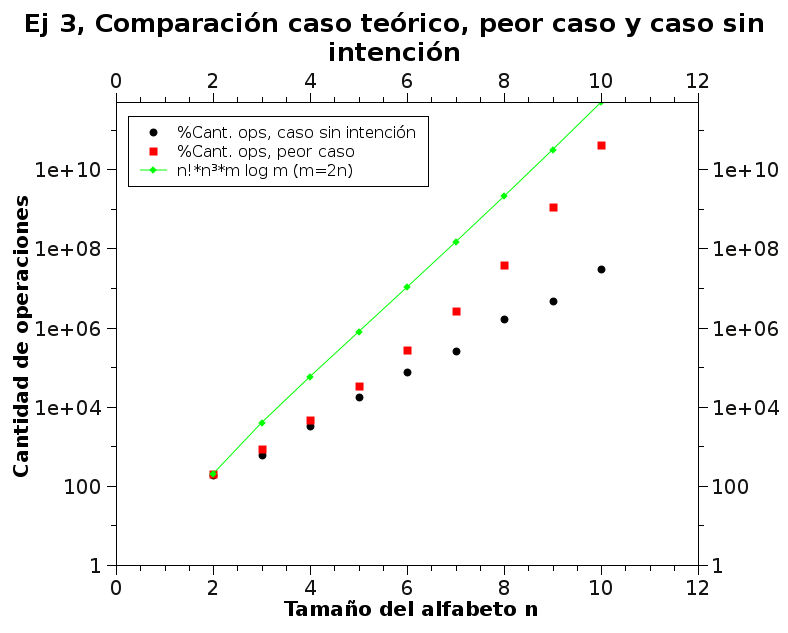
\includegraphics[scale=0.60]{graficos/3-ejG1.png} \\
\scriptsize{\textsf{\textbf{Gr\'afico 3.1}}}  \\
\end{center}

\begin{center}
\begin{tabular}{|c|c|c|}
\hline
\# Tamaño del alfabeto & Cantidad de candidatos al finalizar, con poda & Cantidad de candidatos al finalizar, sin poda\\
\hline
2 & 2 & 2\\
\hline
3 & 2 & 6\\
\hline
4 & 8 & 24\\
\hline
5 & 4 & 120\\
\hline
6 & 4 & 720\\
\hline
7 & 4 & 5,040\\
\hline
8 & 8 & 40,320\\
\hline
9 & 8 & 362,880\\
\hline
10 & 384 & 3,628,800\\
\hline


\end{tabular}
\end{center} \vspace{0,15cm}

Con esta tabla representamos la diferencia que se produce en la cantidad de candidatos generados con poda o sin ella para casos sin intención (un peor caso hace que la poda no corte ningún candidato), es evidente que la poda disminuye notoriamente para estos casos el volumen de datos a procesar, por lo que es muy recomendable implementarla, aún cuando no mejore la complejidad ya que en peor caso no hace nada.

\begin{center}
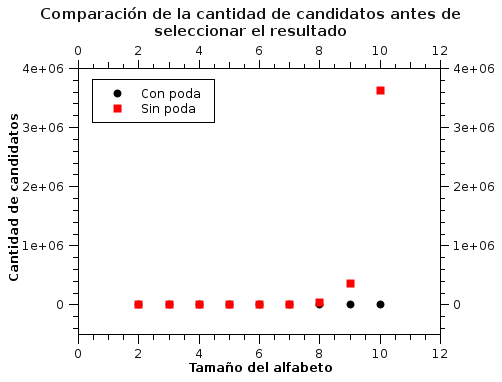
\includegraphics[scale=0.80]{graficos/3-ejG2.png} \\
\scriptsize{\textsf{\textbf{Gr\'afico 3.2}}}  \\
\end{center}


\end{document}
